\documentclass[11pt]{article}

\usepackage[margin=1in]{geometry}
\usepackage{amsmath}
\usepackage{amssymb}
\usepackage[T1]{fontenc}
\usepackage{textcomp}
\usepackage{booktabs}
\usepackage{graphicx}
\usepackage{float}
\usepackage{hyperref}
\usepackage{parskip}

\newcommand{\code}[1]{\texttt{#1}}
\newcommand{\tr}{\operatorname{tr}}

\title{Distribution metrics between a protein and its mutants, decomposed by site and by mode}
\author{Notes for penm}
\date{2026-10-16}

\begin{document}

\maketitle

\section{What is shown}

For every single-point mutant of a complete genm scan, several metrics between the wild type's and
the mutant's Boltzmann distributions are computed and split into per-site and per-mode contributions.
The figures are meant to give a feeling for how the metrics behave; they recommend none.

\paragraph{Data.} 2acy, the genm vignette's wild type (\code{node = "ca"}, \code{model = "ming\_wall"},
$d_{\max}=10.5$\,\AA, \code{d\_max\_graph = 14}, \code{ensemble = 1}, \code{alphabet\_size = 10},
\code{mut\_dl\_sigma = 0.3}, \code{mut\_sd\_min = 2}); all 882 single-point mutants (98 sites, 9 letters
each); $\beta$ at 298\,K. One protein, one model, one ensemble. Scripts: \code{metrics\_scan.R}
(computation) and \code{metrics\_plots.R} (figures and numbers); their printed output is in
\code{metrics\_scan.out.txt} and \code{metrics\_plots.out.txt}.

\section{Definitions}

Both distributions are Gaussians on the wild type's internal subspace; genm superposes the mutant
onto the wild type. In the wild type's mode coordinates ($\mathbf{U}$, $3N\times d$, $d=3N-6=288$):
\[
\mathbf{A}=\operatorname{diag}(\sigma_n^2),\ \sigma_n^2=\frac{1}{\beta\lambda_n};\qquad
\mathbf{B}=\mathbf{U}^T\mathbf{C}^{\rm mut}\mathbf{U};\qquad
\delta\mathbf{r}=\mathbf{U}^T(\mathbf{r}^{\rm mut}-\mathbf{r}^{\rm wt}).
\]
A contribution matrix $\mathbf{M}$ in mode coordinates is attributed to mode $n$ by $M_{nn}$ and to
site $i$ by the trace of the $3\times3$ block of site $i$ in $\mathbf{U}\mathbf{M}\mathbf{U}^T$.
A vector $\mathbf{z}$ is attributed by $z_n^2$ and $|(\mathbf{U}\mathbf{z})_i|^2$.
Both attributions sum to the same total, which the scan checks for every mutant.

\paragraph{Wasserstein-2 (\AA$^2$).}
$W_2^2 = |\delta\mathbf{r}|^2 + \tr\bigl(\mathbf{A}+\mathbf{B}-2(\mathbf{A}^{1/2}\mathbf{B}\mathbf{A}^{1/2})^{1/2}\bigr)$.
It is $E|\mathbf{x}-T(\mathbf{x})|^2$ under the optimal coupling, with
$\mathbf{T}=\mathbf{A}^{-1/2}(\mathbf{A}^{1/2}\mathbf{B}\mathbf{A}^{1/2})^{1/2}\mathbf{A}^{-1/2}$.
Mean part: $\delta\mathbf{r}$, attributed as a vector, so by site it is $|\delta\mathbf{r}_i|^2$
(penm's \code{dr2i}) and by mode $\delta r_n^2$ (\code{dr2n}).
Covariance part: $\mathbf{M}=(\mathbf{I}-\mathbf{T})\mathbf{A}(\mathbf{I}-\mathbf{T})^T$.

\paragraph{Spectral divergences (nats).} With the whitened matrix
$\mathbf{X}=\mathbf{A}^{-1/2}\mathbf{B}\mathbf{A}^{-1/2}=\mathbf{Y}\operatorname{diag}(\nu_k)\mathbf{Y}^T$, the
covariance part of each is $\sum_k g(\nu_k)$, attributed through $\mathbf{M}=\mathbf{Y}\operatorname{diag}(g(\nu_k))\mathbf{Y}^T$:
\begin{center}
\begin{tabular}{lll}
\toprule
divergence & $g(\nu)$ & near $\nu=1+x$ \\
\midrule
KL(mut$\|$wt) & $\tfrac12(\nu-1-\ln\nu)$ & $x^2/4$ \\
Jeffreys (symmetrised KL) & $\tfrac12(\nu+1/\nu-2)$ & $x^2/2$ \\
Bhattacharyya & $\tfrac12\ln\bigl((1+\nu)/(2\sqrt\nu)\bigr)$ & $x^2/16$ \\
affine-invariant (Riemannian), squared & $\ln^2\nu$ & $x^2$ \\
\bottomrule
\end{tabular}
\end{center}
Only the KL mean part is shown: $\tfrac12|\mathbf{A}^{-1/2}\delta\mathbf{r}|^2=\tfrac\beta2\,\delta\mathbf{r}^T\mathbf{K}\delta\mathbf{r}$,
attributed as the vector $\mathbf{A}^{-1/2}\delta\mathbf{r}$; by site this is exactly $\tfrac\beta2\,$\code{de2i}
(checked on one mutant), by mode $\tfrac\beta2\,$\code{de2n}.
Site attribution uses the symmetric square root $\mathbf{C}_{\rm wt}^{-1/2}$, so site shares are in units of the
wild type's own fluctuations.

\paragraph{Frobenius (\AA$^4$, covariance part only).} $\|\mathbf{B}-\mathbf{A}\|_F^2$; by mode
$\sum_m(B-A)_{nm}^2$; by site $\sum_j\|\Delta\mathbf{C}_{ij}\|_F^2$, the row of $3\times3$ blocks of the Cartesian
difference, so correlations with other sites count.

\paragraph{Sums of marginal divergences.} KL and $W_2^2$ between the $3\times3$ marginals of each site,
and between the one-dimensional marginals along each wild-type mode, means included. These add up by
construction, but their sum is not the divergence between the full distributions.

\paragraph{penm.} \code{dmsfi}$^2$ and \code{dmsfn}$^2$, squared as in the genm vignette.

\section{Results}

\subsection{Averages over the scan, by site and by mode}

\begin{figure}[H]
\centering
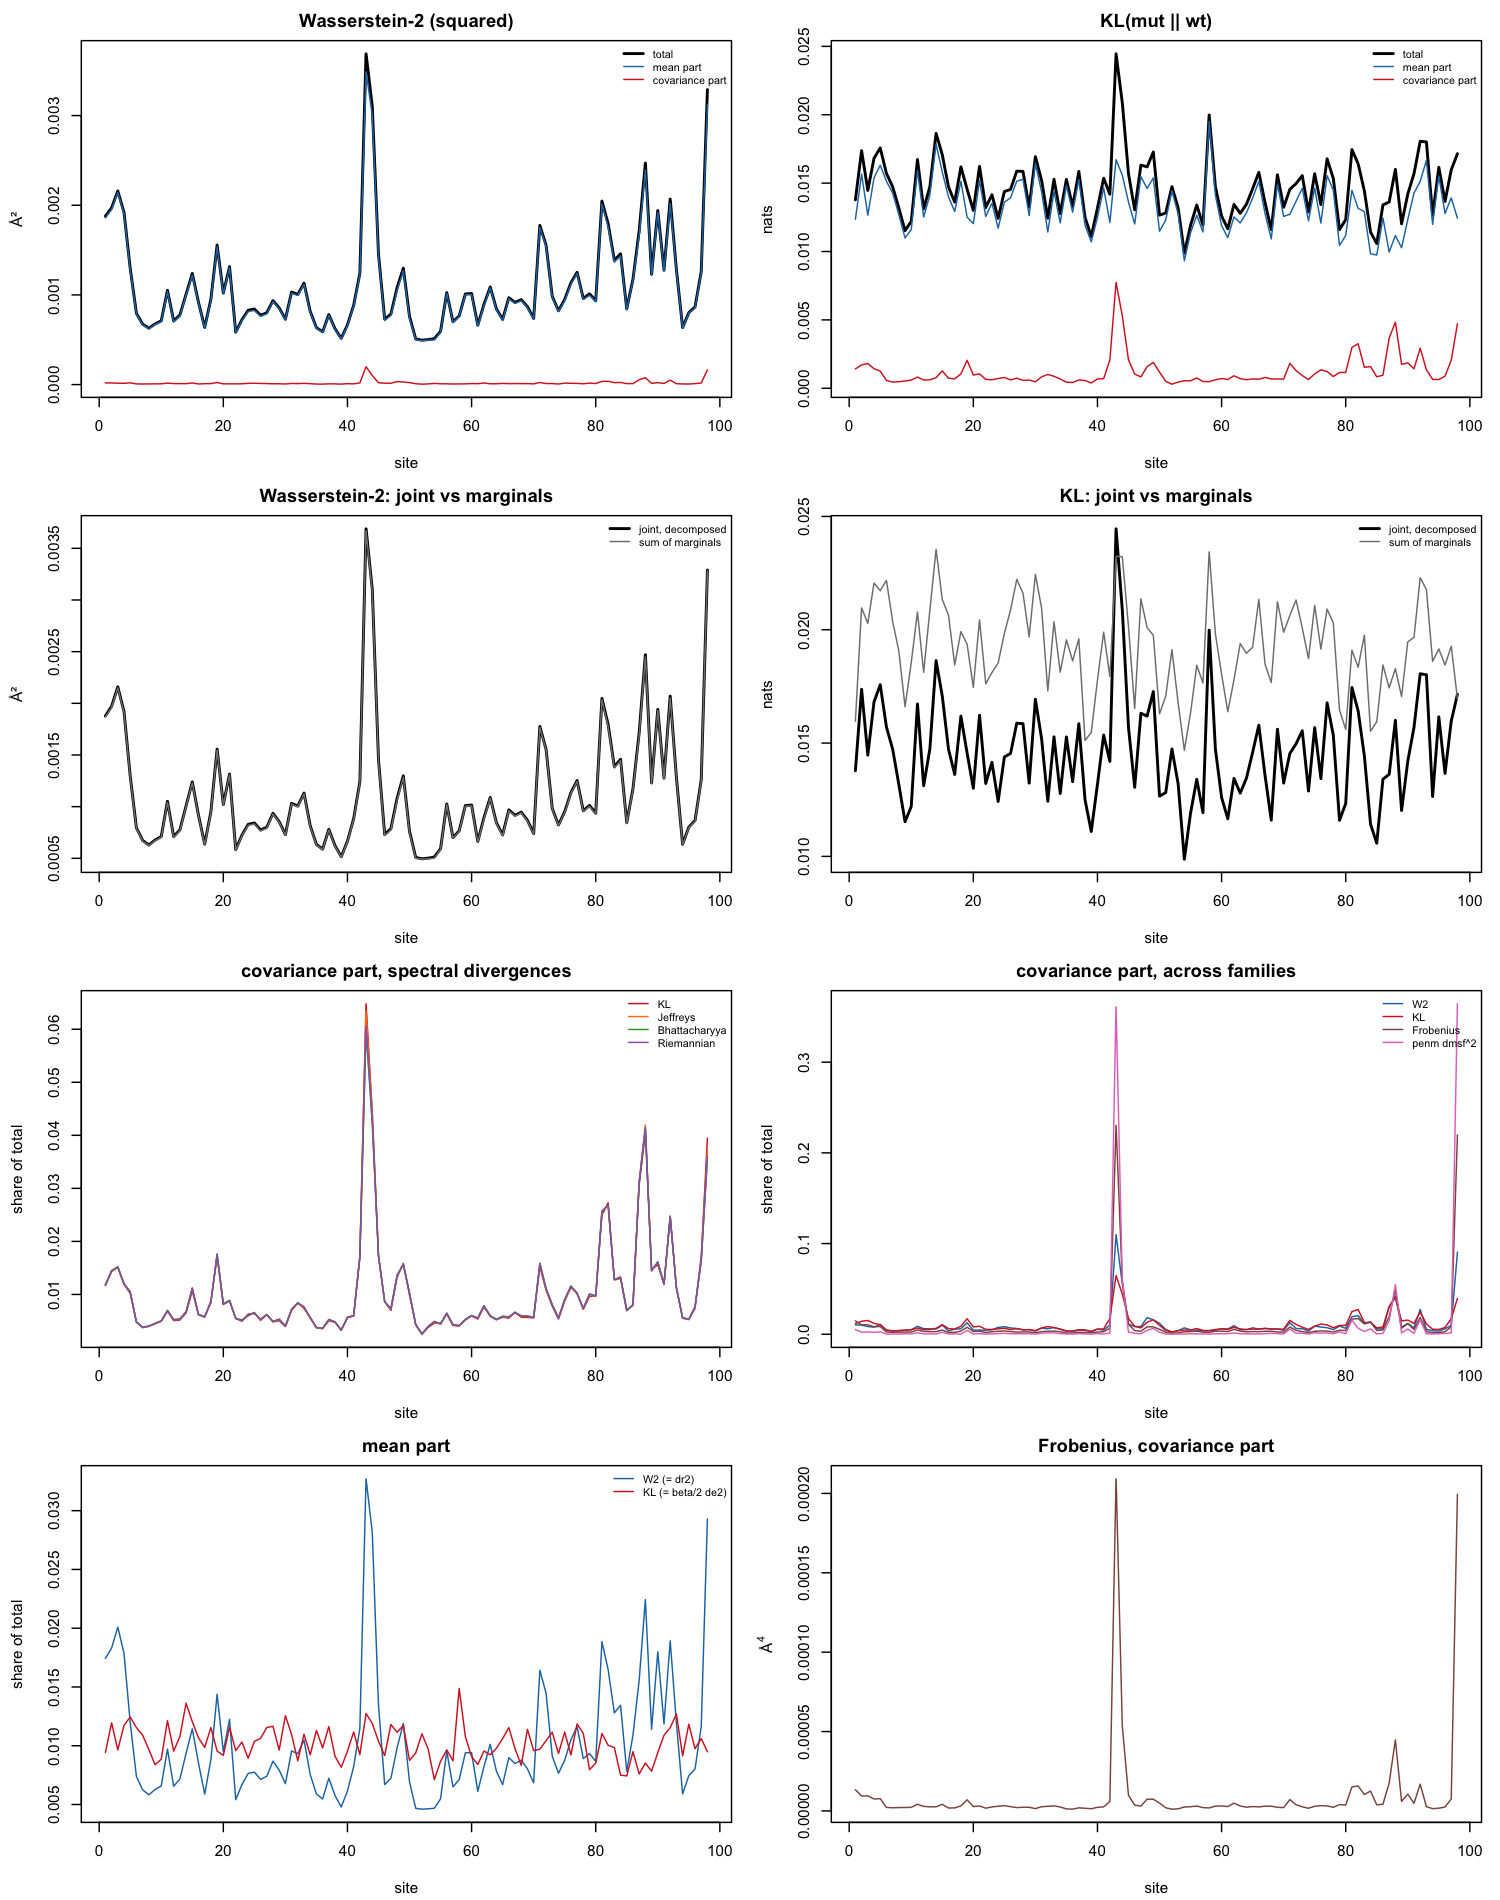
\includegraphics[width=0.92\textwidth]{metrics_by_site.png}
\caption{Means over the 882 mutants, by site. ``Share of total'' panels divide each profile by its sum,
to compare shapes across units.}
\label{fig:site}
\end{figure}

\begin{figure}[H]
\centering
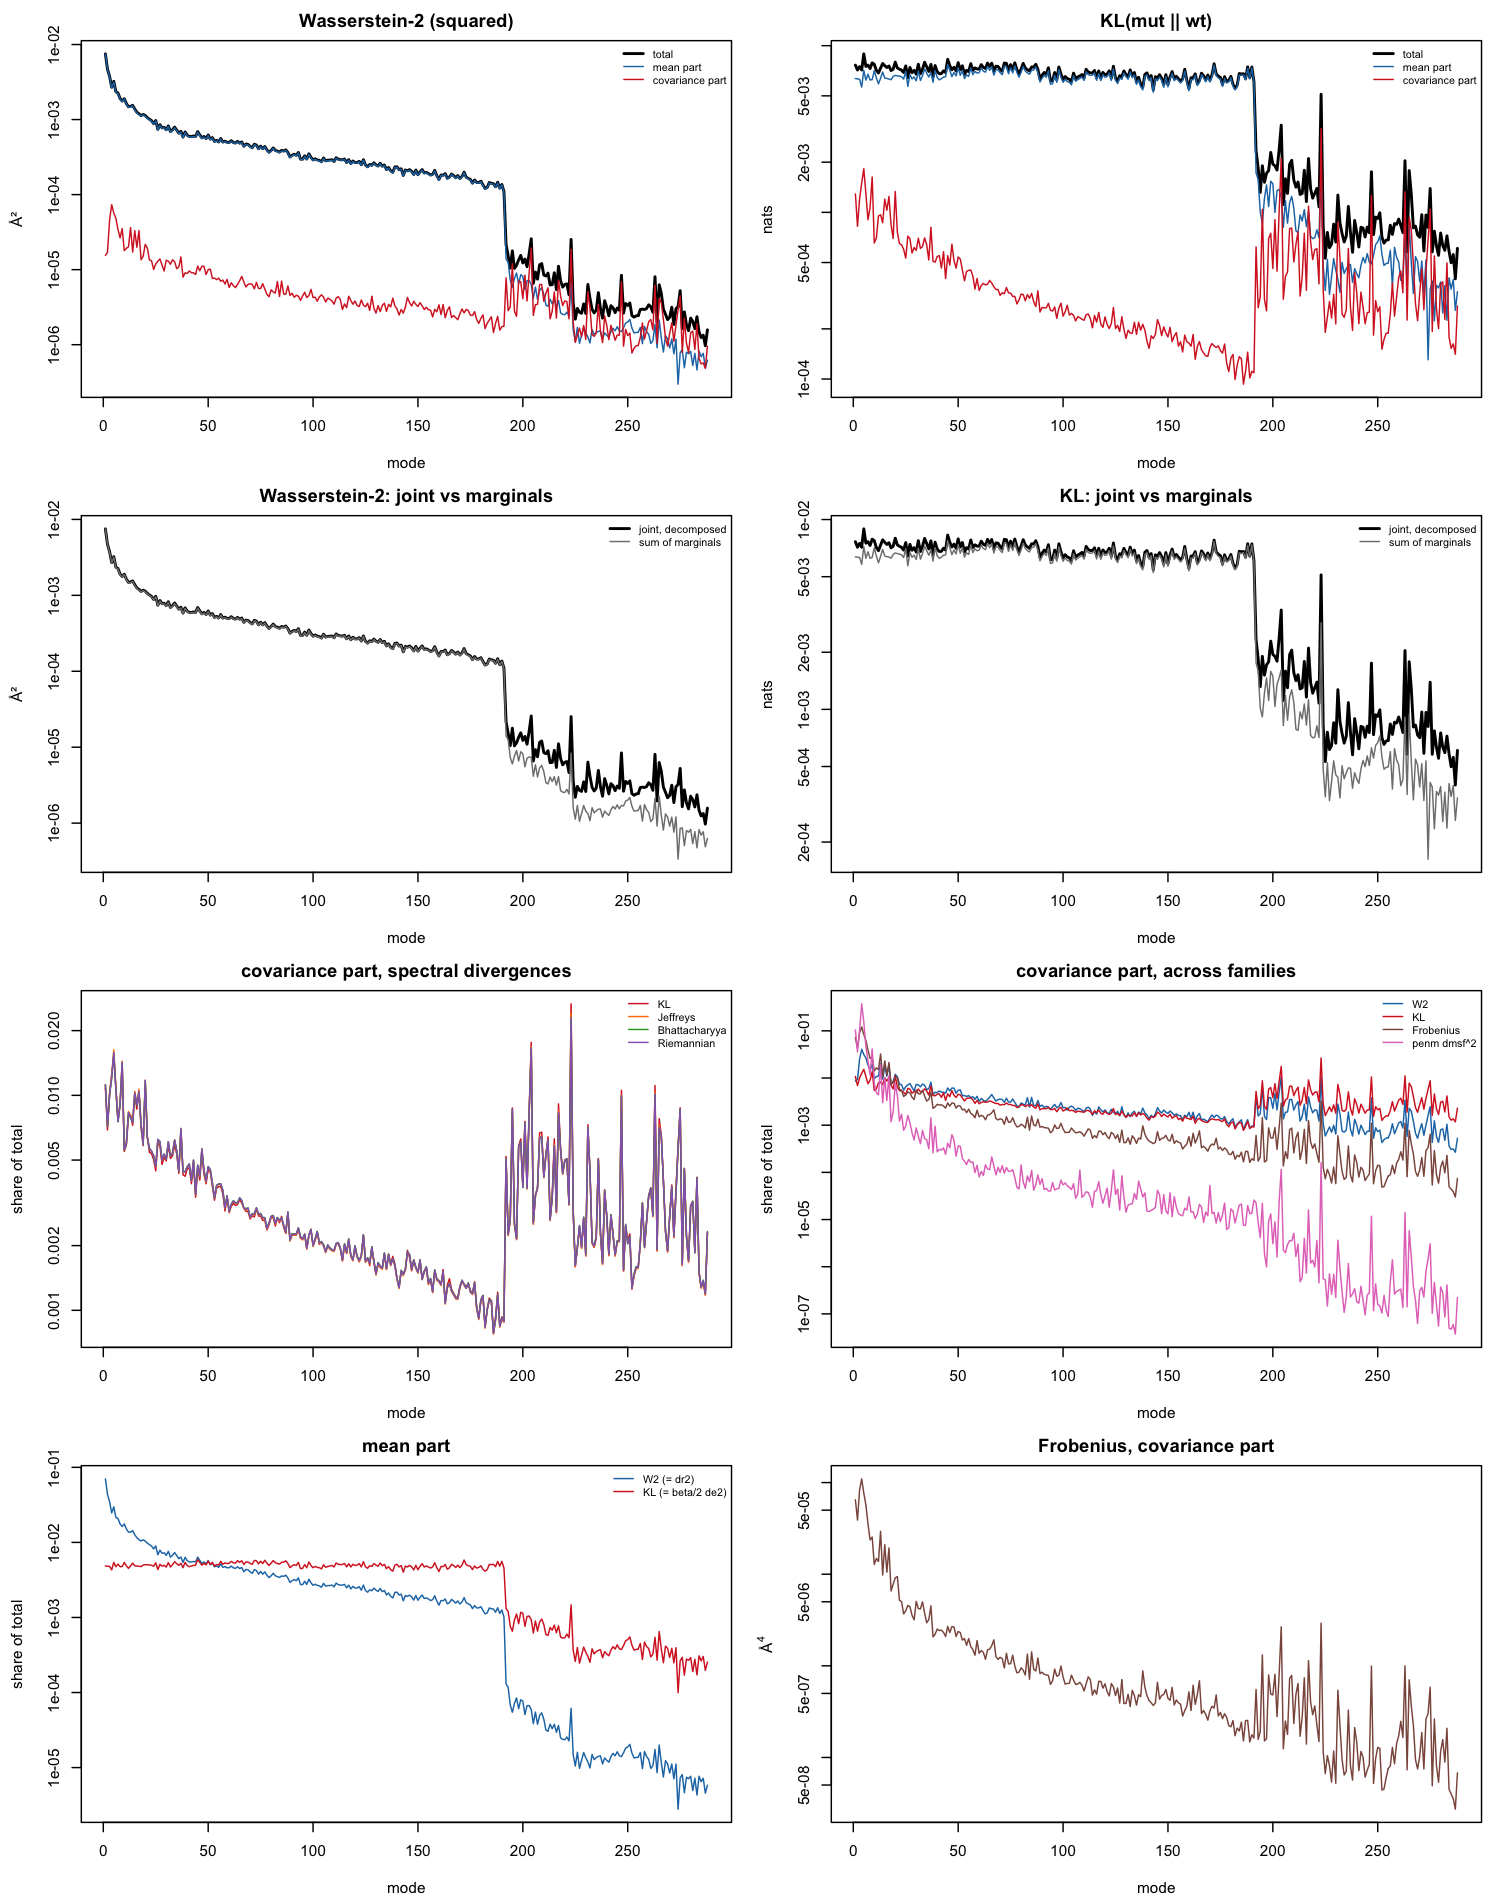
\includegraphics[width=0.92\textwidth]{metrics_by_mode.png}
\caption{As Figure~\ref{fig:site}, by wild-type mode; logarithmic vertical axes.}
\label{fig:mode}
\end{figure}

What the two figures show:
\begin{itemize}
\item \textbf{Mean parts dominate.} Median over mutants of the covariance part's share of the total:
  1.0\% for $W_2^2$, 7.2\% for KL. Across mutants the KL mean and covariance parts correlate
  (Spearman 0.58).
\item \textbf{$W_2$ weighs by displacement, KL by energy.} The $W_2$ mean part by site is
  \code{dr2i}: largest at the flexible sites (around 43--44, the C terminus, 80--98). The KL mean part
  by site, $\tfrac\beta2$\code{de2i}, is nearly flat. The two site profiles have Spearman 0.22.
  By mode, $W_2$ falls with mode index (soft modes move most), while the KL mean part is nearly flat
  across the lower band: there $\tfrac12\delta r_n^2/\sigma_n^2$ is about constant, so the mutational
  displacements along the lower-band modes scale like the thermal variances $\sigma_n^2$.
  Both drop at the band gap (mode 191/192).
\item \textbf{The four spectral divergences give the same profiles.} Their scan-mean profiles have
  Spearman 1.00 with each other, by site and by mode. Near $\nu=1$ all four $g$ are proportional to
  $(\nu-1)^2$; over all mutants $\nu$ ranges over 0.24--4.4, but the median over mutants of the largest
  $|\nu-1|$ is 0.32.
\item \textbf{Covariance parts across families.} By site, the covariance parts of $W_2$, KL, Frobenius and
  \code{dmsf}$^2$ peak at the same sites (43 and 98 above all), with Spearman 0.86--0.91, but differ in how
  concentrated they are: the shares of sites 43 and 98 are 0.36 each for \code{dmsf}$^2$, 0.23 and 0.22
  for Frobenius, 0.11 and 0.09 for $W_2$, while KL's largest shares are 0.065 (site 43) and 0.044 (site 44). By mode they differ more: $W_2$, Frobenius and \code{dmsf}$^2$ fall with mode
  index, \code{dmsf}$^2$ by about five orders of magnitude, while KL is flatter and rises in the upper band
  (Spearman of KL with \code{dmsf}$^2$ by mode: 0.42).
\item \textbf{Joint against marginals.} For $W_2$, the per-site attribution of the joint and the sum of
  site marginals nearly coincide: the mean part is the same in both, $|\delta\mathbf{r}_i|^2$, and the
  covariance part is small. For KL, the sum of site marginals exceeds the joint (median ratio 1.27) and
  its site profile follows the KL mean part (Spearman 0.87) but not the joint covariance part (0.13):
  each marginal weights $\delta\mathbf{r}_i$ by its own block $\mathbf{C}_{ii}^{-1}$, not by the joint's
  $\mathbf{K}$.
\end{itemize}

\begin{figure}[H]
\centering
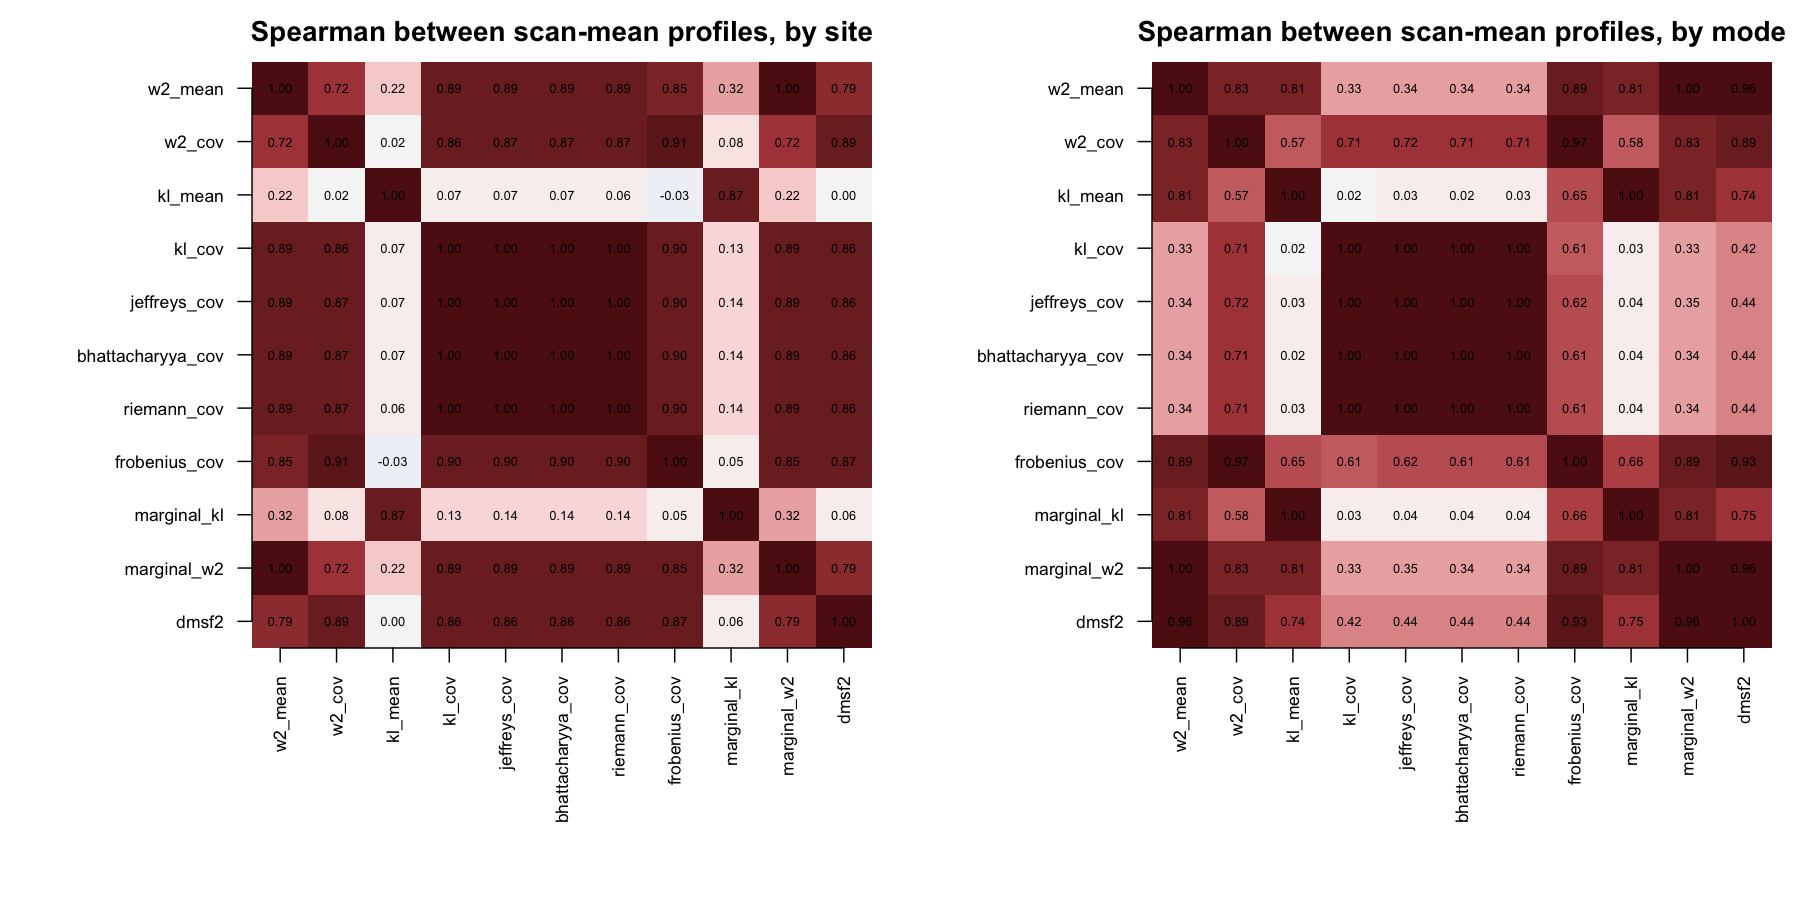
\includegraphics[width=\textwidth]{metrics_correlations.png}
\caption{Spearman correlations between the scan-mean profiles of all components, by site (left) and by
mode (right).}
\label{fig:cor}
\end{figure}

\subsection{Individual mutants}

\begin{figure}[H]
\centering
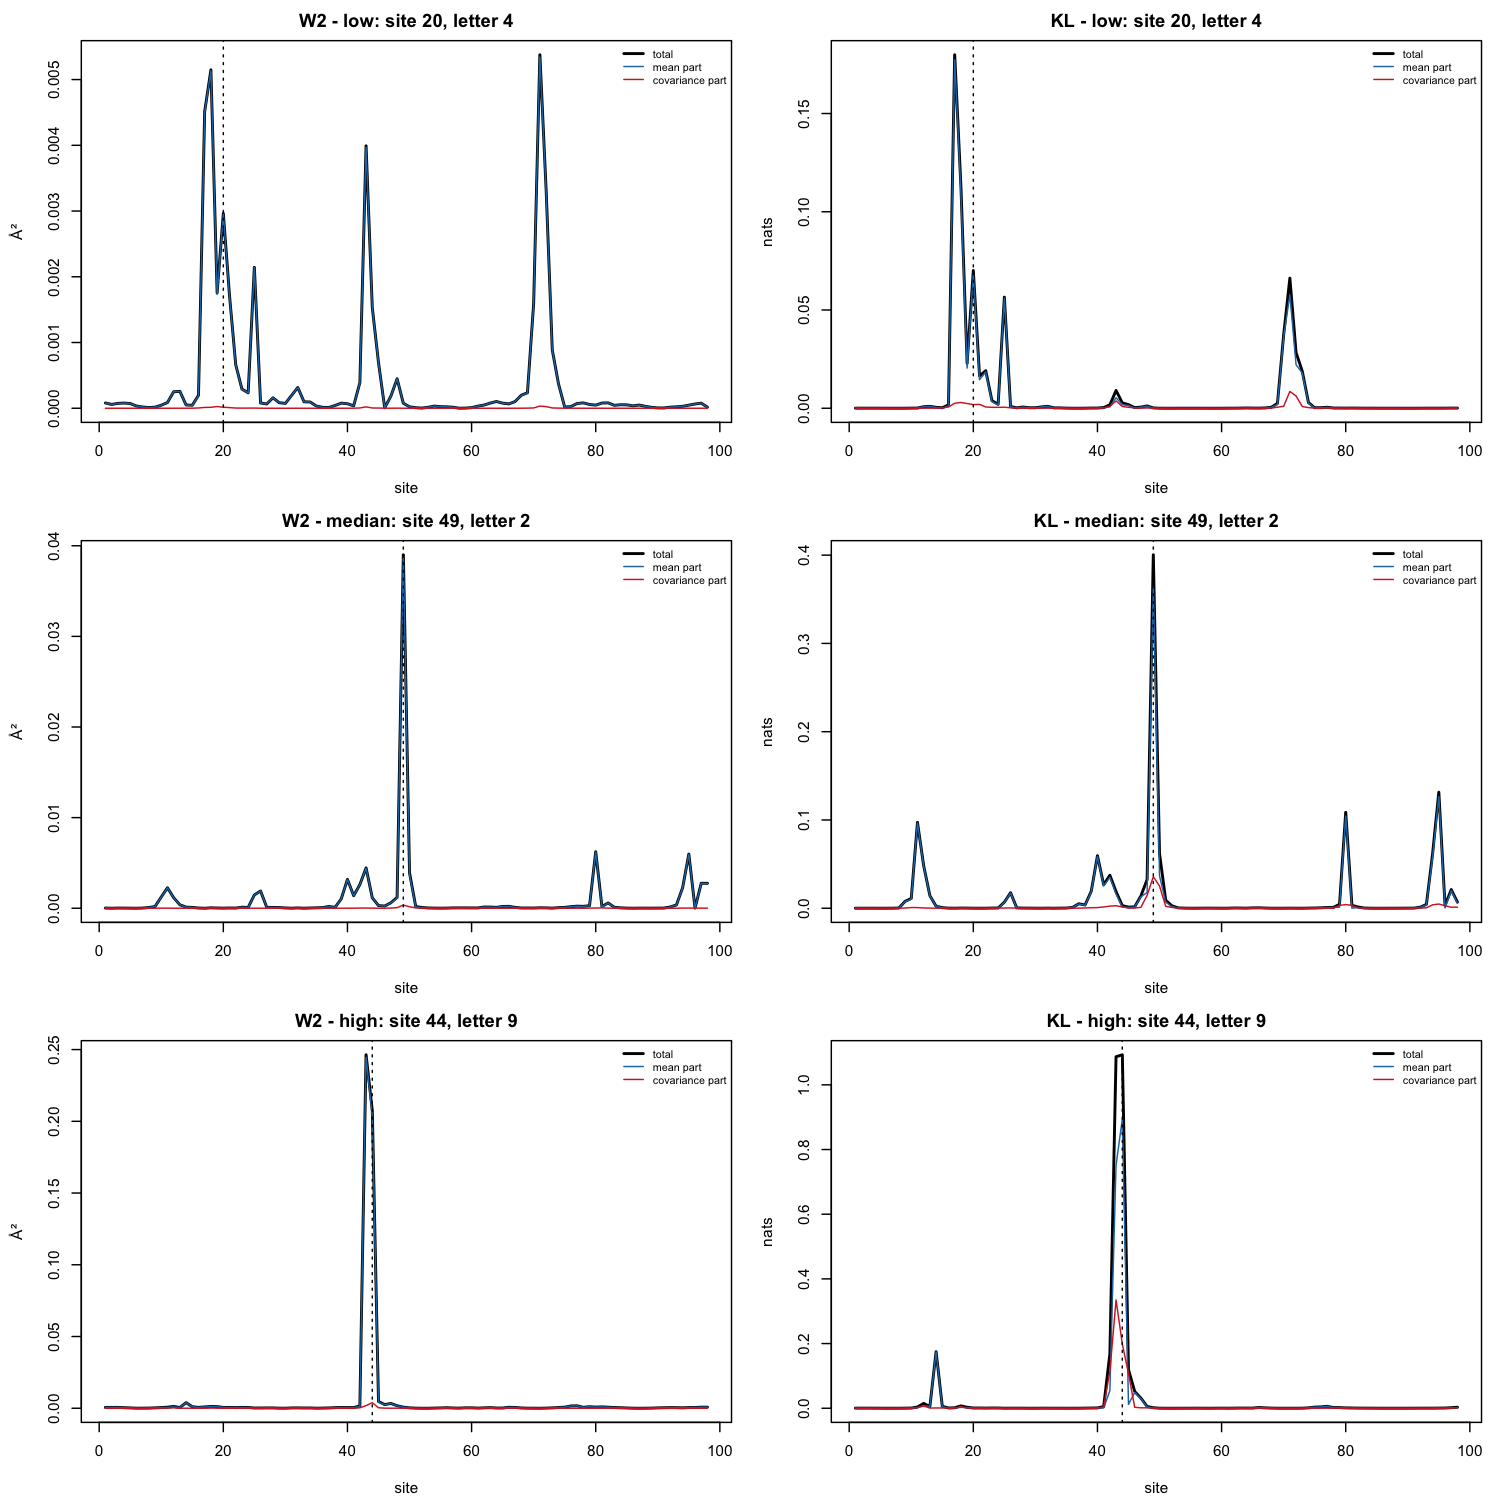
\includegraphics[width=0.92\textwidth]{metrics_examples.png}
\caption{Site profiles of $W_2^2$ and KL for three mutants: the 10th percentile (site 20, letter 4),
the median (site 49, letter 2) and the largest (site 44, letter 9) of $W_2^2$. The dotted line marks the
mutated site.}
\label{fig:examples}
\end{figure}

Single mutants have localised profiles: the mutated site and a few others. $W_2$ and KL agree on where
the peaks are but not on their heights; in the 10th-percentile mutant, the peaks near sites 18 and 71 are
about equal in $W_2$, while in KL the one near 17--18 is nearly three times the one at 71. The covariance
part is visible only in KL, and mostly next to the mutated site (in the largest mutant, about 0.33 nats at
site 43).

\subsection{Totals over mutants}

\begin{figure}[H]
\centering
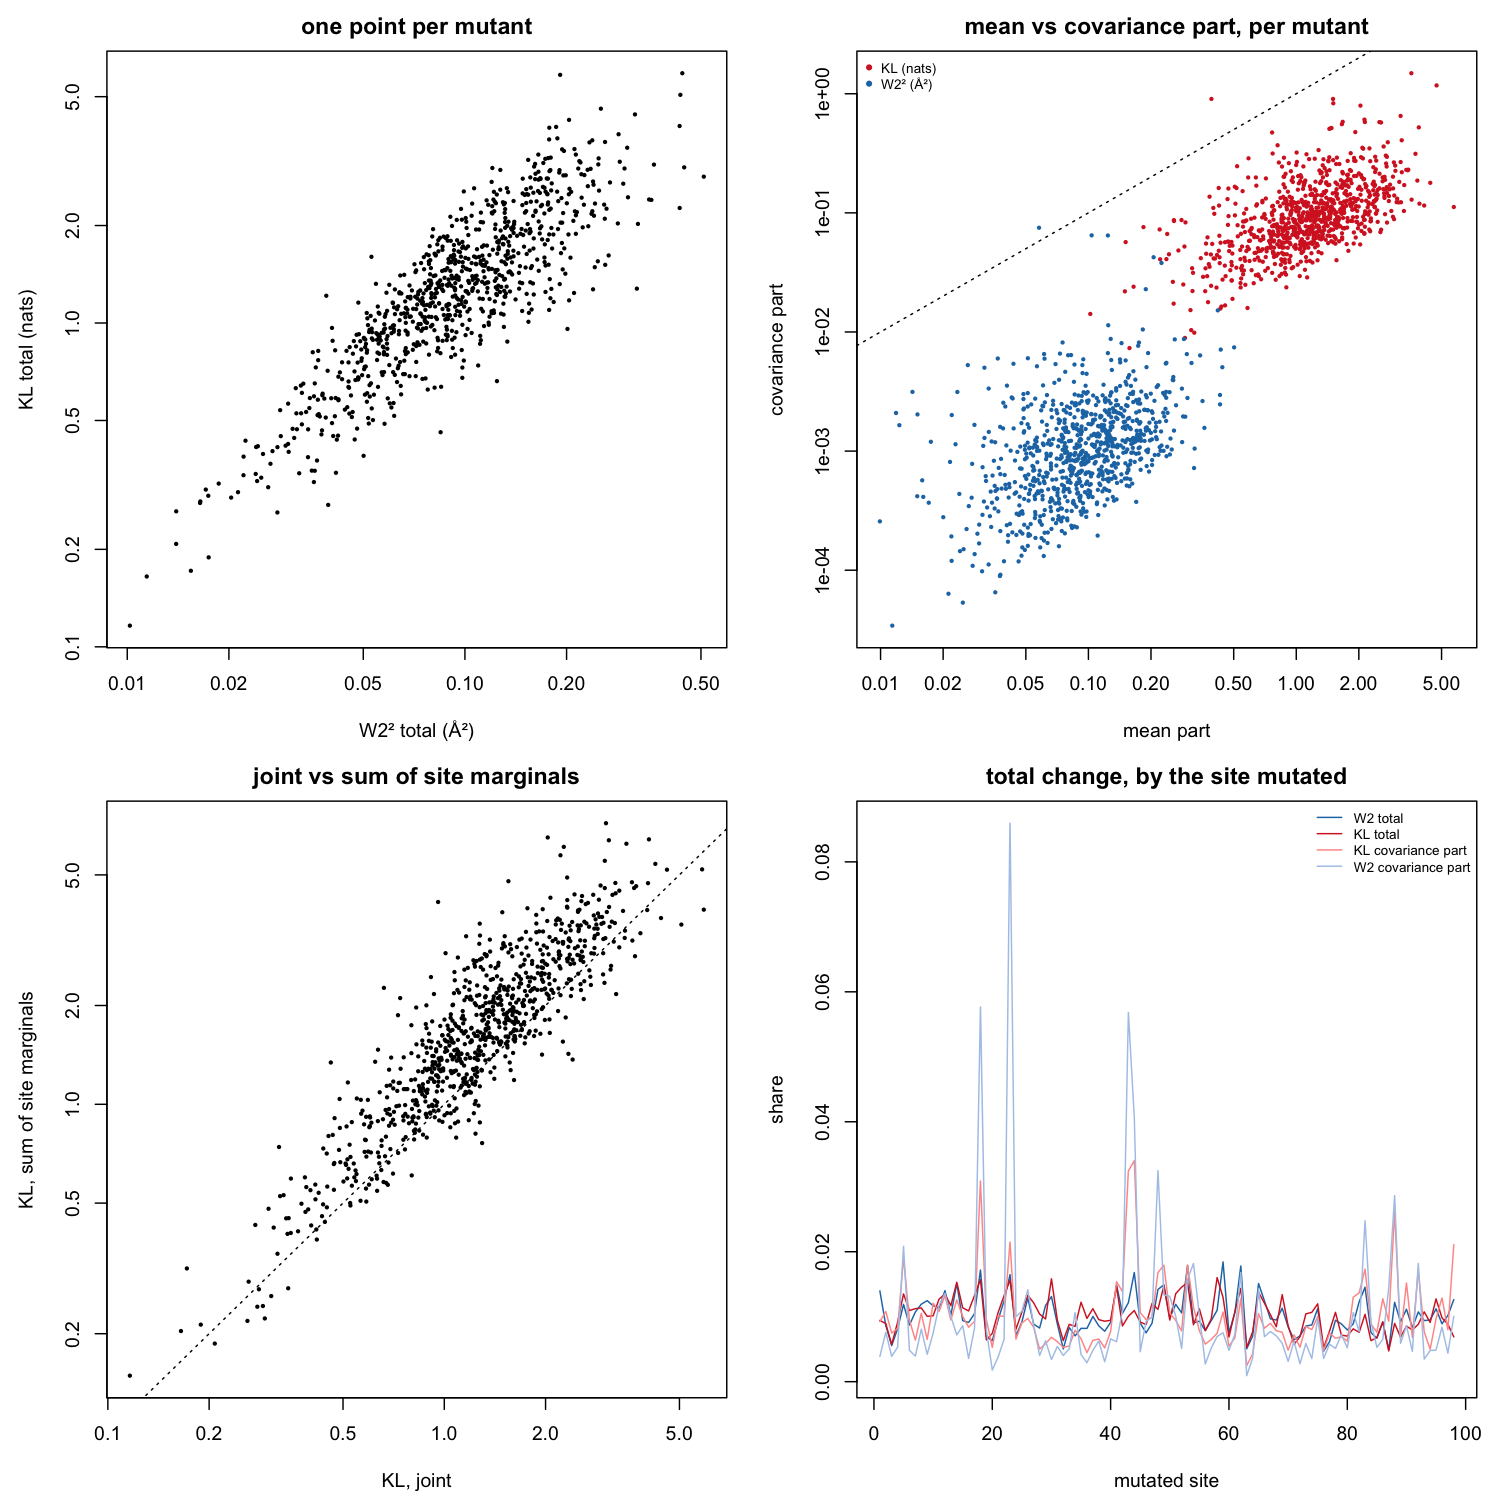
\includegraphics[width=0.92\textwidth]{metrics_totals.png}
\caption{Top left: KL against $W_2^2$, one point per mutant. Top right: covariance part against mean part,
for both. Bottom left: KL between the full distributions against the sum of site-marginal KLs; the dotted
line is equality. Bottom right: each total averaged over the nine mutations at each site, as a share of its
sum.}
\label{fig:totals}
\end{figure}

\begin{itemize}
\item Global totals: $W_2^2$ median 0.093\,\AA$^2$ (mean part) and 0.0011\,\AA$^2$ (covariance part);
  KL median 1.17 and 0.091 nats.
\item The two totals rank mutants similarly (Spearman 0.84).
\item Averaged by the mutated site, the totals are fairly even across sites; the covariance parts are not:
  in the figure, $W_2$'s covariance part is largest for mutations around sites 18, 23, 43--44, 48, 83 and 88.
\end{itemize}

\section{Things to keep in mind}

\begin{itemize}
\item Under lfenm the covariance is unchanged, so every covariance part is zero and each metric reduces
  to its mean part.
\item The KL and spectral attributions to sites depend on choosing the symmetric square root for whitening;
  $W_2$'s and Frobenius's do not involve a choice.
\item Every comparison is made in the wild type's internal subspace, after genm's superposition.
\item One protein, one elastic network model, one ensemble of mutations.
\end{itemize}

\end{document}
